\documentclass{article}
\usepackage{amsthm,amsmath,amsfonts,lipsum}
\usepackage[T1]{fontenc}
\usepackage{beramono}
\usepackage{listings}
\usepackage{fontawesome5}
\usepackage{adjustbox}
\usepackage{mathabx}
\usepackage{thmtools}
\usepackage{import}
\usepackage{graphicx}
\usepackage{setspace}
\usepackage{geometry}
\usepackage{physics}
\usepackage{float}
\usepackage[english]{babel}
\usepackage{framed}
\usepackage[dvipsnames,x11names]{xcolor}
\usepackage{tcolorbox}
\usepackage{fancyhdr}
\usepackage{hyperref}
\usepackage{booktabs}
\usepackage{enumitem}
\usepackage{cancel}
\usepackage{background}
\usepackage{units}

% Configuring the background
\backgroundsetup{
  scale=1, % Optional, scale if needed
  color=black, % Optional, set the image color, can be omitted
  opacity=0.18, % Optional, adjust opacity for watermark effect
  angle=0,
  position=current page.center, % Center the image on the page
  contents={
\includegraphics[width=1.75\paperwidth, height=1.75\paperheight, keepaspectratio]{ninym_ralei_leaf (watermarked by AlexanderTheMango)}} % Keeps aspect ratio and scales to fill the page
}

% Colours
\definecolor{darkgreen}{rgb}{0.0, 0.5, 0.0}
\definecolor{Firebrick}{rgb}{0.698, 0.132, 0.203}
\definecolor{Crimson}{rgb}{0.862745, 0.078431, 0.235294} % Crimson color
\definecolor{lightred}{rgb}{1.0, 0.819608, 0.819608} % Light red for background
\definecolor{MediumPurple}{rgb}{0.576, 0.439, 0.859}
\definecolor{chocolate}{rgb}{0.82, 0.41, 0.12} % Chocolate color definition
% Define the Navy color
\definecolor{Navy}{rgb}{0.0, 0.0, 0.5}

% Define custom tcolorbox styles for notes
\tcbuselibrary{skins, breakable}
\newtcolorbox{definitionbox}{colframe=RoyalBlue, colback=blue!5!white, title=Definition}
\newtcolorbox{examplebox}{colframe=ForestGreen, colback=green!5!white, title=Example}
\newtcolorbox{notebox}{colframe=RedOrange, colback=orange!5!white, title=Note}
\newtcolorbox{theorembox}{colframe=RoyalPurple, colback=purple!5!white, title=Theorem}

\newtcolorbox{propositionbox}{colframe=Goldenrod, colback=yellow!10!white, title=Proposition}
\newtcolorbox{remarkbox}{colframe=MidnightBlue, colback=blue!10!white, title=Remark}
\newtcolorbox{corollarybox}{colframe=OliveGreen, colback=green!10!white, title=Corollary}
\newtcolorbox{warningbox}{colframe=Crimson, colback=lightred, title=Warning}
\newtcolorbox{proofbox}{colframe=Black, colback=gray!10!white, title=Proof}
\newtcolorbox{questionbox}{colframe=Teal, colback=teal!10!white, title=Question}
\newtcolorbox{tipbox}{colframe=Goldenrod, colback=yellow!10!white, title=Tip}
\newtcolorbox{exercisebox}{colframe=darkgreen, colback=green!5!white, title=Exercise}
\newtcolorbox{solutionbox}{colframe=DodgerBlue4, colback=blue!5!white, title=Solution}
\newtcolorbox{algorithmbox}{colframe=Navy, colback=blue!10!white, title=Algorithm}
\newtcolorbox{conceptbox}{colframe=chocolate, colback=brown!10!white, title=Concept}
\newtcolorbox{illustrationbox}{colframe=Firebrick, colback=red!10!white, title=Illustration}
\newtcolorbox{intuitionbox}{colframe=MediumPurple, colback=purple!10!white, title=Intuition}
\newtcolorbox{answerbox}{colframe=RoyalBlue, colback=blue!10!white, title=Answer}

% Geometry settings
\geometry{letterpaper, portrait, includeheadfoot=true, hmargin=1in, vmargin=1in}
\onehalfspacing

% Header and footer
\pagestyle{fancy}
\fancyhf{}
\lhead{MAT232 - Lecture Notes}
\rhead{\thepage}
\lfoot{University of Toronto Mississauga}
\rfoot{\today}

% Document starts
\begin{document}
\renewcommand{\familydefault}{\rmdefault}

\begin{titlepage}
    \null % This is a TeX command that does nothing but is necessary for vfill to work correctly
    \vfill
    \begin{center}
        {\fontsize{40}{48}\selectfont \bfseries MAT232 - Lecture 13}
        \vspace{20pt} \\
        {\LARGE after partial derivatives?} \\
        \vspace{20pt}
        \textbf{AlexanderTheMango}
        \vspace{8pt}
        \\ Prepared for February 24, 2025
    \end{center}
    \vfill
\end{titlepage}


\newpage
\tableofcontents
\newpage

\begin{titlepage}
    \null % Ensures proper alignment with vfill
    \vfill
    \begin{center}
        {\Huge \textbf{Definitions and Theorems}} \\[20pt]
        \rule{\textwidth}{0.5mm} \\[15pt]
        {\Large \textit{Straight from the textbook — lots of fluff this time, more than what we need!}} \\[15pt]
        \rule{\textwidth}{0.5mm} \\[15pt]
        \textbf{Quick recap before diving into the lecture.}
    \end{center}
    \vfill
\end{titlepage}


\section*{Preliminary Definitions and Theorems}
\addcontentsline{toc}{section}{Preliminary Definitions and Theorems}

% Definition: Polar Coordinates
\begin{definitionbox}
\textbf{Polar Coordinates.} \\
Each point in the Cartesian plane can be represented in polar coordinates as an ordered pair $(r, \theta)$, where $r$ is the radial coordinate (distance from the origin), and $\theta$ is the angular coordinate (angle measured from the positive $x$-axis).  
The correspondence between Cartesian coordinates $(x, y)$ and polar coordinates $(r, \theta)$ is given by:
\[
x = r\cos\theta, \quad y = r\sin\theta, \quad r^2 = x^2 + y^2, \quad \tan\theta = \frac{y}{x}.
\]
\end{definitionbox}

% Theorem: Converting Points
\begin{theorembox}
\textbf{Theorem 1.4. Converting Points Between Coordinate Systems.} \\
Given a point $P$ in the plane with Cartesian coordinates $(x, y)$ and polar coordinates $(r, \theta)$, the following conversion formulas hold true:
\[
x = r\cos\theta, \quad y = r\sin\theta,
\]
\[
r^2 = x^2 + y^2, \quad \tan\theta = \frac{y}{x}.
\]
These formulas can be used to convert between Cartesian and polar coordinates.
\end{theorembox}

% Example: Converting Coordinates
\begin{examplebox}
\textbf{Example 1.10. Converting Between Rectangular and Polar Coordinates.}
\begin{enumerate}
    \item Convert $(1, 1)$ to polar coordinates:  
    Use $x = 1$ and $y = 1$. Then:
    \[
    r^2 = x^2 + y^2 = 1^2 + 1^2 = 2 \implies r = \sqrt{2}, \quad \tan\theta = \frac{y}{x} = \frac{1}{1} = 1 \implies \theta = \frac{\pi}{4}.
    \]
    Therefore, $(1, 1)$ can be represented as $(\sqrt{2}, \dfrac{\pi}{4})$ in polar coordinates.
\end{enumerate}
\end{examplebox}

% Problem-Solving Strategy: Plotting a Curve
\begin{conceptbox}
\textbf{Problem-Solving Strategy: Plotting a Curve in Polar Coordinates.}
\begin{enumerate}
    \item Create a table with two columns: one for $\theta$ values and one for $r$ values.
    \item Calculate the corresponding $r$ values for each $\theta$.
    \item Plot each ordered pair $(r, \theta)$ on the polar coordinate axes.
    \item Connect the points and observe the resulting graph.
\end{enumerate}
\end{conceptbox}

% Example: Graphing in Polar Coordinates
\begin{examplebox}
\textbf{Example 1.12. Graphing a Function in Polar Coordinates.} \\
Graph the curve defined by $r = 4\sin\theta$.  
\begin{enumerate}
    \item Create a table of values for $\theta$ and calculate $r$:
    \[
    \begin{array}{c|c|c|c|c|c|c}
    \theta & 0 & \frac{\pi}{6} & \frac{\pi}{4} & \frac{\pi}{2} & \pi & 2\pi \\
    \hline
    r = 4\sin\theta & 0 & 2 & 2\sqrt{2} & 4 & 0 & 0
    \end{array}
    \]
    \item Plot the points and connect them to form the curve. The result is a circle with radius $2$ centered at $(0, 2)$ in rectangular coordinates.
\end{enumerate}
\begin{figure}[H]
    \centering
    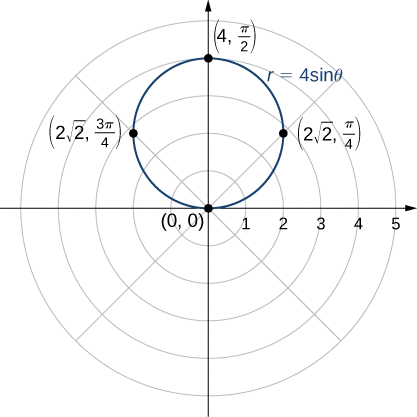
\includegraphics[width=0.5\textwidth]{rEquals4sinTheta.png}
    \caption{The graph of the function \( r = 4\sin\theta \) is a circle.}
    \label{fig:sample_image}
\end{figure}
\end{examplebox}

\begin{titlepage}
    \null % Ensures proper alignment with vfill
    \vfill
    \begin{center}
        {\Huge \textbf{Let’s Get Started}} \\[20pt]
        \rule{\textwidth}{0.5mm} \\[15pt]
        {\Large \textit{Time to dive into the lecture notes.}} \\[15pt]
        \rule{\textwidth}{0.5mm} \\[15pt]
        \textbf{Grab your pen or pencil, and let’s break this down step by step.}
    \end{center}
    \vfill
\end{titlepage}

\normalsize

\section*{Recall: 1st Year Calculus}
\addcontentsline{toc}{section}{The Definite Integral}
\begin{definitionbox}
The \textbf{definite integral} of a function \( y = f(x) \), where \( f(x) \geq 0 \), represents the area under the curve from \( x = a \) to \( x = b \):
\[
    \text{Area} = \int_{x=a}^{x=b} f(x) \, dx
\]
\begin{figure}[H]
    \centering
    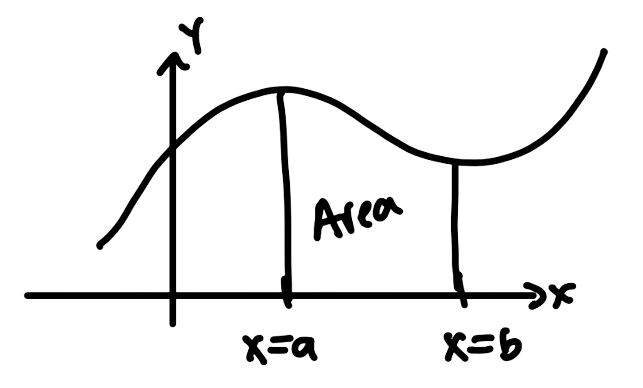
\includegraphics[width=0.6\textwidth]{1styearcalc.jpg}
    \caption{Illustration of the area under \( y = f(x) \).}
    \label{fig:sample_image}
\end{figure}
\end{definitionbox}

\section*{Section 1.2: Area Enclosed by a Parametric Curve}
\addcontentsline{toc}{section}{The Area Under a Parametric Curve}
\begin{definitionbox}
A \textbf{parametric curve} is defined by:
\[
    x = f(t), \quad y = g(t), \quad \alpha \leq t \leq \beta
\]
with the following properties:
\begin{itemize}
    \item The curve lies above the \( x \)-axis.
    \item The curve does not self-intersect.
\end{itemize}
\begin{figure}[H]
    \centering
    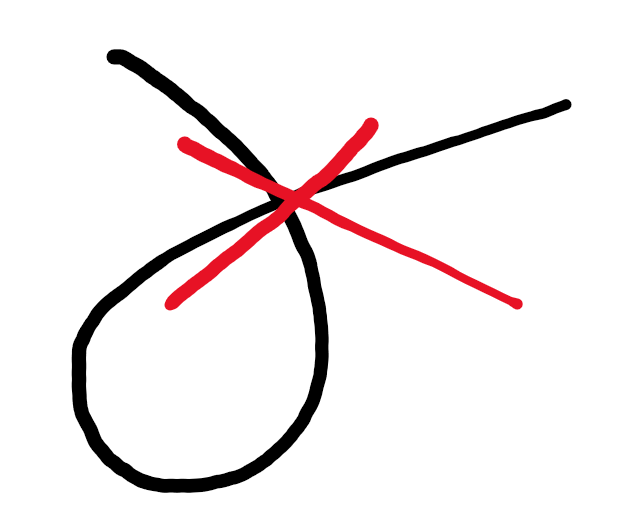
\includegraphics[width=0.15\textwidth]{self_intersecting_parametric_curve_example.png}
    \caption{A curve that self-intersects.}
    \label{fig:sample_image}
\end{figure}

\begin{theorembox}
    The area enclosed by the curve is given by:
    \[
        \text{Area} = \int_{t=\alpha}^{t=\beta} g(t) f'(t) \, dt
    \]
    or equivalently:
    \[
        \text{Area} = \int_{t=\alpha}^{t=\beta} f(t) g'(t) \, dt
    \]
\end{theorembox}
\end{definitionbox}

\subsection*{Alternative Forms for Area}
\begin{notebox}
In specific cases, the area can also be calculated using:
\[
    \text{Area} = \int_{y=c}^{y=d} x(y) \, dy
\]
or:
\[
    \text{Area} = \int_{x=a}^{x=b} y(x) \, dx
\]
\end{notebox}

\section*{Example: Standard Parametric Curve}
\addcontentsline{toc}{subsection}{Example: Standard Parametric Curve}
\begin{examplebox}
Calculate the area enclosed by the parametric curve:
\[
    x = \cos(t), \quad y = \sin(t), \quad 0 \leq t \leq \pi
\]

\begin{solutionbox}
The area is calculated as:
\[
    \text{Area} = \int_{t=\alpha}^{t=\beta} g(t) f'(t) \, dt,
\]
where \( x = f(t) \) and \( y = g(t) \). Here, \( f(t) = \cos(t) \), \( g(t) = \sin(t) \), and \( f'(t) = -\sin(t) \). Substituting:
\[
    \text{Area} = \int_{t=0}^{t=\pi} \sin(t)(-\sin(t)) \, dt = \int_{t=0}^{t=\pi} -\sin^2(t) \, dt.
\]

Using \( \sin^2(t) = \frac{1}{2}(1 - \cos(2t)) \), we get:
\[
    \text{Area} = -\int_{t=0}^{t=\pi} \frac{1}{2}(1 - \cos(2t)) \, dt = -\frac{1}{2} \left[ \int_{t=0}^{t=\pi} 1 \, dt - \int_{t=0}^{t=\pi} \cos(2t) \, dt \right].
\]

Evaluate the integrals:
\[
    \int_{t=0}^{t=\pi} 1 \, dt = \pi, \quad \int_{t=0}^{t=\pi} \cos(2t) \, dt = \left[ \frac{\sin(2t)}{2} \right]_0^\pi = 0.
\]

Thus:
\[
    \text{Area} = -\frac{1}{2}(\pi - 0) = -\frac{\pi}{2}.
\]
Taking the absolute value (since area is positive):
\[
    \text{Area} = \frac{\pi}{2}.
\]
\end{solutionbox}
\end{examplebox}

\section*{Example: Cycloid}
\addcontentsline{toc}{subsection}{Example: Cycloid}
\begin{examplebox}
\textbf{Example:} Find the area under the cycloid defined by:
\[
    x = t - \sin(t), \quad y = 1 - \cos(t), \quad 0 \leq t \leq 2\pi.
\]

\begin{solutionbox}
The area under a parametric curve is given by:
\[
    \text{Area} = \int_{t=\alpha}^{t=\beta} g(t) f'(t) \, dt, \quad f'(t) = \frac{dx}{dt}.
\]
\\
\textbf{Step 1: Substitution} \\
From \( x = t - \sin(t) \) and \( y = 1 - \cos(t) \):  
\[
    f'(t) = 1 - \cos(t), \quad g(t) = 1 - \cos(t).
\]
Substitute into the formula:
\[
    \text{Area} = \int_{0}^{2\pi} (1 - \cos(t))^2 \, dt.
\]
\\
\textbf{Step 2: Expand and Separate Terms} \\
Expand \( (1 - \cos(t))^2 \):
\[
    \text{Area} = \int_{0}^{2\pi} [1 - 2\cos(t) + \cos^2(t)] \, dt.
\]
Split the integral:
\[
    \text{Area} = \int_{0}^{2\pi} 1 \, dt - 2\int_{0}^{2\pi} \cos(t) \, dt + \int_{0}^{2\pi} \cos^2(t) \, dt.
\]
\textit{...cont'd...}
\end{solutionbox}
\end{examplebox}
\begin{examplebox}
\begin{solutionbox}
\textit{...cont'd...} \\
\\
\textbf{Step 3: Evaluate Each Term} \\
1. \underline{First Term:}  
\[
    \int_{0}^{2\pi} 1 \, dt = 2\pi.
\]  
2. \underline{Second Term:}  
\[
    \int_{0}^{2\pi} \cos(t) \, dt = [\sin(t)]_{0}^{2\pi} = 0.
\]  
3. \underline{Third Term:} \\
\\
Using \( \cos^2(t) = \dfrac{1 + \cos(2t)}{2} \):  
\[
    \int_{0}^{2\pi} \cos^2(t) \, dt = \frac{1}{2} \int_{0}^{2\pi} 1 \, dt + \frac{1}{2} \int_{0}^{2\pi} \cos(2t) \, dt.
\]
Evaluate:  
\[
    \frac{1}{2} \int_{0}^{2\pi} 1 \, dt = \pi, \quad \frac{1}{2} \int_{0}^{2\pi} \cos(2t) \, dt = 0.
\]
Thus:
\[
    \int_{0}^{2\pi} \cos^2(t) \, dt = \pi.
\]

\textbf{Step 4: Combine Results}  
\[
    \text{Area} = 2\pi - 0 + \pi = 3\pi.
\]

\begin{answerbox}
\( \text{Area} = 3\pi \) 
\end{answerbox}

\end{solutionbox}
\end{examplebox}


\section*{Homework Practice Question: Area Under a Parametric Curve}
\addcontentsline{toc}{subsection}{Homework Practice Question}
\begin{exercisebox}
    Find the area under the curve defined by
    \[
        x = 3\cos(t) + \cos(3t), \quad y = 3\sin(t) - \sin(3t), \quad 0 \leq t \leq \pi.
    \]
    Hint: Recall that \( \sin^2(x) + \cos^2(x) = 1 \).
    
    \begin{solutionbox}
    The area under a parametric curve is given by:
    \[
        \text{Area} = \int_{t=\alpha}^{t=\beta} g(t) f'(t) \, dt,
    \]
    where \( x = f(t) \), \( y = g(t) \), and \( f'(t) = \frac{dx}{dt} \). \\
    \\
    \textbf{Step 1: Differentiate \( x(t) \)} \\
    Given \( x = 3\cos(t) + \cos(3t) \), compute:
    \[
        f'(t) = \frac{d}{dt}[3\cos(t) + \cos(3t)] = -3\sin(t) - 3\sin(3t).
    \]
    \\
    \textbf{Step 2: Substitute into the Formula} \\
    The parametric area formula becomes:
    \[
        \text{Area} = \int_{0}^{\pi} \big[3\sin(t) - \sin(3t)\big] \big[-3\sin(t) - 3\sin(3t)\big] \, dt.
    \]
    \\
    \textbf{Step 3: Simplify the Expression} \\
    Expand the product:
    \[
        \big[3\sin(t) - \sin(3t)\big]\big[-3\sin(t) - 3\sin(3t)\big] = -9\sin^2(t) - 9\sin(t)\sin(3t) + 3\sin(3t)\sin(t) + 3\sin^2(3t).
    \]
    Combine terms:
    \[
        -9\sin^2(t) + 3\sin^2(3t) - 6\sin(t)\sin(3t).
    \]
    \textit{...cont'd...}
    \end{solutionbox}
\end{exercisebox}
\begin{exercisebox}
    \begin{solutionbox}
    \textit{...cont'd..} \\

    Using the product-to-sum identity for \( \sin(a)\sin(b) = \frac{1}{2}[\cos(a-b) - \cos(a+b)] \):
    \[
        \sin(t)\sin(3t) = \frac{1}{2}[\cos(2t) - \cos(4t)].
    \]
        
    Substitute this back:
    \[
        \text{Area} = \int_{0}^{\pi} \big[-9\sin^2(t) + 3\sin^2(3t) - 3[\cos(2t) - \cos(4t)]\big] \, dt.
    \]
    \\
    \textbf{Step 4: Break the Integral into Separate Terms} \\
    Split the integral:
    \[
        \text{Area} = -9\int_{0}^{\pi} \sin^2(t) \, dt + 3\int_{0}^{\pi} \sin^2(3t) \, dt - 3\int_{0}^{\pi} \cos(2t) \, dt + 3\int_{0}^{\pi} \cos(4t) \, dt.
    \]

    \textbf{Step 5: Evaluate Each Integral}  

    1. \underline{First Term (\(-9\int_{0}^{\pi} \sin^2(t) \, dt\)):} \\
    \\
       Use the identity \( \sin^2(t) = \dfrac{1 - \cos(2t)}{2} \):
       \[
           \int_{0}^{\pi} \sin^2(t) \, dt = \int_{0}^{\pi} \frac{1 - \cos(2t)}{2} \, dt = \frac{1}{2} \int_{0}^{\pi} 1 \, dt - \frac{1}{2} \int_{0}^{\pi} \cos(2t) \, dt.
       \]
       Evaluate:
       \[
           \frac{1}{2} \int_{0}^{\pi} 1 \, dt = \frac{\pi}{2}, \quad \frac{1}{2} \int_{0}^{\pi} \cos(2t) \, dt = \frac{1}{2}[0] = 0.
       \]
       So:
       \[
           \int_{0}^{\pi} \sin^2(t) \, dt = \frac{\pi}{2}.
       \]
       Multiply by \(-9\):
       \[
           -9\int_{0}^{\pi} \sin^2(t) \, dt = -9 \cdot \frac{\pi}{2} = -\frac{9\pi}{2}.
       \]
    \textit{...cont'd...}
    \end{solutionbox}
\end{exercisebox}
\begin{exercisebox}
    \begin{solutionbox}
        \textit{...cont'd...} \\
        \\
        2. \underline{Second Term (\(3\int_{0}^{\pi} \sin^2(3t) \, dt\)):} \\
        \\
       Similarly, \( \sin^2(3t) = \dfrac{1 - \cos(6t)}{2} \):
       \[
           \int_{0}^{\pi} \sin^2(3t) \, dt = \frac{1}{2} \int_{0}^{\pi} 1 \, dt - \frac{1}{2} \int_{0}^{\pi} \cos(6t) \, dt.
       \]
       Evaluate:
       \[
           \frac{1}{2} \int_{0}^{\pi} 1 \, dt = \frac{\pi}{2}, \quad \frac{1}{2} \int_{0}^{\pi} \cos(6t) \, dt = 0.
       \]
       So:
       \[
           \int_{0}^{\pi} \sin^2(3t) \, dt = \frac{\pi}{2}.
       \]
       Multiply by 3:
       \[
           3\int_{0}^{\pi} \sin^2(3t) \, dt = 3 \cdot \frac{\pi}{2} = \frac{3\pi}{2}.
       \]

    3. \underline{Third Term (\(-3\int_{0}^{\pi} \cos(2t) \, dt\)):} \\
    \\
       Since \(\int_{0}^{\pi} \cos(2t) \, dt = 0\):
       \[
           -3\int_{0}^{\pi} \cos(2t) \, dt = 0.
       \]

    4. \underline{Fourth Term (\(3\int_{0}^{\pi} \cos(4t) \, dt\)):} \\
    \\
       Similarly, \(\int_{0}^{\pi} \cos(4t) \, dt = 0\):
       \[
           3\int_{0}^{\pi} \cos(4t) \, dt = 0.
       \]
    \\
    \textbf{Step 6: Combine Results} \\
    Add the evaluated terms:
    \[
        \text{Area} = -\frac{9\pi}{2} + \frac{3\pi}{2} + 0 + 0 = -\frac{6\pi}{2} = -3\pi.
    \]
    However, the area is always positive, so:
    \[
        \text{Area} = 3\pi.
    \]
    \end{solutionbox}
\end{exercisebox}
\begin{exercisebox}
    \begin{solutionbox}
        \textit{...cont'd...}
        \begin{answerbox}
            \( \text{Area} = 3\pi \)
        \end{answerbox}
    \end{solutionbox}
\end{exercisebox}

\section*{The Arc Length of a Parametric Curve}
\addcontentsline{toc}{section}{The Arc Length of a Parametric Curve}

\begin{theorembox}

    Let a curve be parameterized by \( t \), such that:
    \[
    x = x(t) \quad \text{and} \quad y = y(t), \quad \text{for } t \in [\alpha, \beta].
    \]
    
    The \textbf{arc length} \( L \) of the curve between \( t = \alpha \) and \( t = \beta \) is given by:
    \[
        L = \int_{t=\alpha}^{t=\beta} \sqrt{\left(\frac{dx}{dt}\right)^2 + \left(\frac{dy}{dt}\right)^2} \, dt
    \]

\begin{conceptbox}
Consider two points \( (x_1, y_1) \) and \( (x_2, y_2) \) on a curve. The differences in their coordinates are defined as:
\[ \Delta x = x_2 - x_1, \quad \Delta y = y_2 - y_1 \]

The distance \( D \) between the two points is given by the Pythagorean theorem:
\[
    D = \sqrt{(x_2 - x_1)^2 + (y_2 - y_1)^2}
\]
Substituting \( \Delta x \) and \( \Delta y \):
\[
    D = \sqrt{\Delta x^2 + \Delta y^2}
\]

Now, consider the curve parameterized by \( t \), where \( x = x(t) \) and \( y = y(t) \). Dividing \( \Delta x \) and \( \Delta y \) by the parameter \( \Delta t \):
\[
    D \approx \sqrt{\left(\frac{\Delta x}{\Delta t}\right)^2 + \left(\frac{\Delta y}{\Delta t}\right)^2} \Delta t
\]

Taking the limit as \( \Delta t \to 0 \), this becomes a Riemann sum. Therefore, the arc length \( L \) of the curve is:
\[
    L = \int_{t=\alpha}^{t=\beta} \sqrt{\left(\frac{dx}{dt}\right)^2 + \left(\frac{dy}{dt}\right)^2} \, dt
\]
\end{conceptbox}

\begin{notebox}
    \( L \) represents the total length of the curve between \( t = \alpha \) and \( t = \beta \). This formula is provided on the formula sheet for term test 1.
\end{notebox}
\end{theorembox}

\begin{illustrationbox}
    \begin{figure}[H]
        \centering
        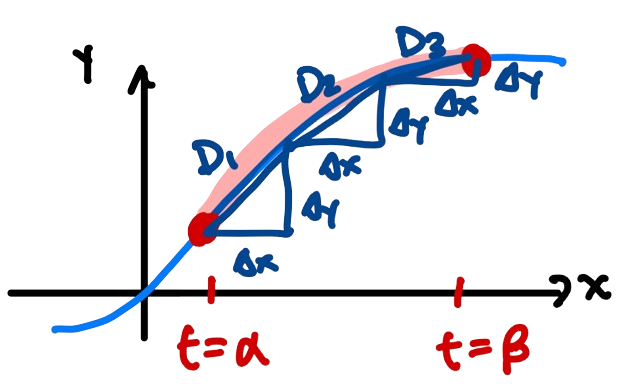
\includegraphics[width=0.6\textwidth]{arc length riemann sums showcase}
        \caption{Visualizing the arc length theorem — the connection between Riemann sums and the integral for a curve's length.}
        \label{fig:sample_image1}
    \end{figure}
\end{illustrationbox}

\section*{Example: Parametric Curve}
\addcontentsline{toc}{subsection}{Example: Parametric Curve}
\begin{examplebox}
    Find the arc length of the curve defined by:
    \[
        x = 3\cos(t), \quad y = 3\sin(t), \quad t \in [0, 2\pi].
    \]
    
    \begin{solutionbox}
        The arc length is denoted by \( L \). We evaluate it as follows:

        \begin{equation*}
            \begin{aligned}
                L &= \int_{0}^{2\pi} \sqrt{\left(\frac{dx}{dt}\right)^2 + \left(\frac{dy}{dt}\right)^2} dt \\
                &= \int_{0}^{2\pi} \sqrt{\left(-3\sin(t)\right)^2 + \left(3\cos(t)\right)^2} dt \\
                &= \int_{0}^{2\pi} \sqrt{9\sin^2(t) + 9\cos^2(t)} dt.
            \end{aligned}
        \end{equation*}
    
        Using the Pythagorean identity \( \sin^2(t) + \cos^2(t) = 1 \), simplify the integrand:
    
        \begin{equation*}
            \begin{aligned}
                L &= \int_{0}^{2\pi} \sqrt{9 \cdot (\sin^2(t) + \cos^2(t))} dt \\
                &= \int_{0}^{2\pi} \sqrt{9 \cdot 1} \, dt \\
                &= \int_{0}^{2\pi} 3 \, dt.
            \end{aligned}
        \end{equation*}
    
        The integral simplifies to:
    
        \begin{equation*}
            \begin{aligned}
                L &= 3 \int_{0}^{2\pi} 1 \, dt \\
                &= 3 \left[t\right]_{0}^{2\pi} \\
                &= 3 \cdot \left(2\pi - 0\right) \\
                &= 6\pi.
            \end{aligned}
        \end{equation*}
        \begin{answerbox}
            The arc length of the curve is \( L = 6\pi \).
        \end{answerbox}
    \end{solutionbox}
\end{examplebox}

\section*{Homework Practice Problem: Parametric Curve}
\addcontentsline{toc}{subsection}{Homework Practice Problem: Parametric Curve}
\begin{notebox}
    Find the arc length of the curve defined by:
    \[
        x = 3t^2, \quad y = 2t^3, \quad 1 \leq t \leq 3.
    \]

    \begin{solutionbox}
        The arc length is denoted by \( L \), which is evaluated as follows:

    \begin{equation*}
        \begin{aligned}
            L &= \int_{1}^{3} \sqrt{\left(\frac{dx}{dt}\right)^2 + \left(\frac{dy}{dt}\right)^2} dt.
        \end{aligned}
    \end{equation*}

    Compute the derivatives:
    \[
        \frac{dx}{dt} = \frac{d}{dt}(3t^2) = 6t, \quad \frac{dy}{dt} = \frac{d}{dt}(2t^3) = 6t^2.
    \]

    Substitute these into the arc length formula:
    \begin{equation*}
        \begin{aligned}
            L &= \int_{1}^{3} \sqrt{(6t)^2 + (6t^2)^2} dt \\
            &= \int_{1}^{3} \sqrt{36t^2 + 36t^4} dt \\
            &= \int_{1}^{3} \sqrt{36t^2(1 + t^2)} dt \\
            &= \int_{1}^{3} 6t\sqrt{1 + t^2} dt.
        \end{aligned}
    \end{equation*}

    Use substitution to simplify the integral. Let:
    \[
        u = 1 + t^2, \quad \frac{du}{dt} = 2t, \quad dt = \frac{du}{2t}.
    \]

    Change the limits of integration:
    \[
        \text{When } t = 1, \, u = 1 + 1^2 = 2; \quad \text{When } t = 3, \, u = 1 + 3^2 = 10.
    \]

    Substitute into the integral:
    \begin{equation*}
        \begin{aligned}
            L &= \int_{2}^{10} 6t \cdot \sqrt{u} \cdot \frac{du}{2t} \\
            &= \int_{2}^{10} 3\sqrt{u} \, du.
        \end{aligned}
    \end{equation*}
    \end{solutionbox}
\end{notebox}
\begin{notebox}
    \begin{solutionbox}
        Evaluate the integral:
        \begin{equation*}
            \begin{aligned}
                L &= 3 \int_{2}^{10} u^{1/2} \, du \\
                &= 3 \left[\frac{2}{3} u^{3/2} \right]_{2}^{10} \\
                &= 2 \left[u^{3/2}\right]_{2}^{10} \\
                &= 2 \left[(10)^{3/2} - (2)^{3/2}\right].
            \end{aligned}
        \end{equation*}
    
        Simplify the result:
        \[
            L = 2 \left[10\sqrt{10} - 2\sqrt{2}\right].
        \]
    
        \begin{answerbox}
            The arc length of the curve is \( L = 2 \left(10\sqrt{10} - 2\sqrt{2}\right) \).
        \end{answerbox}
    \end{solutionbox}
\end{notebox}

\section*{Section 1.3: Polar Coordinates}
\addcontentsline{toc}{section}{Polar Coordinates}

\begin{definitionbox}
\textbf{Polar coordinates} represent a point in the plane by specifying its distance from the origin (\( r \)) and the angle (\( \theta \)) it makes with the positive x-axis, measured counterclockwise.

\vspace{0.5em}

\begin{conceptbox}
    \textbf{Cartesian Coordinates:}
    \begin{figure}[H]
        \centering
        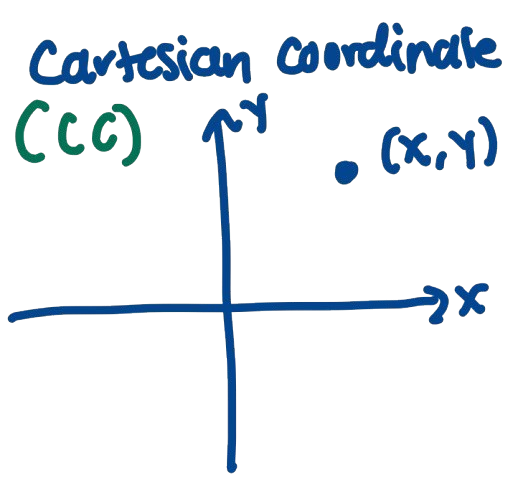
\includegraphics[width=0.4\textwidth]{cartesian.png}
        \caption{Graphical representation of Cartesian coordinates.}
        \label{fig:cartesian_coordinates}
    \end{figure}
    
    \textbf{Polar Coordinates:}
    \begin{figure}[H]
        \centering
        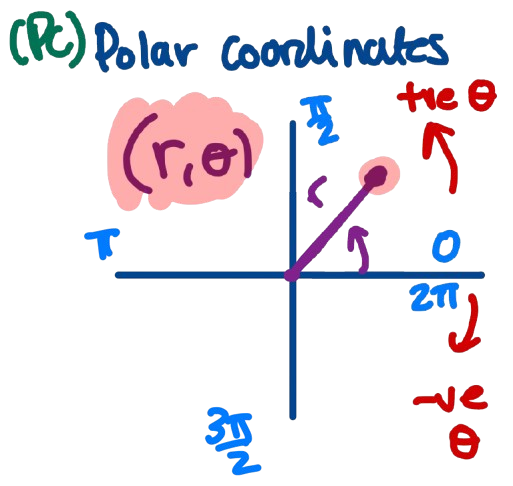
\includegraphics[width=0.4\textwidth]{polar.png}
        \caption{Graphical representation of Polar coordinates.}
        \label{fig:polar_coordinates}
    \end{figure}
\end{conceptbox}
\end{definitionbox}

\section*{How to Work with Polar Coordinates}
\addcontentsline{toc}{subsection}{How to Work with Polar Coordinates}

\begin{tipbox}
    \begin{enumerate}
        \item Start from the origin and move radially outward by a distance equal to \( r \).
        \item From this position, rotate the point counterclockwise by an angle \( \theta \) (in radians or degrees).
        \item The resultant position is the point represented by the polar coordinate \( (r, \theta) \).
    \end{enumerate}
    
    \vspace{1em}
    
    \subsection*{Converting from Cartesian to Polar Coordinates}
    \begin{algorithmbox}
    
        \begin{enumerate}
            \item Given a point \( (x, y) \) in Cartesian coordinates:
                  \[
                  r = \sqrt{x^2 + y^2}, \quad \theta = \tan^{-1}\left(\frac{y}{x}\right).
                  \]
            \item \( r \) represents the radial distance from the origin.
            \item \( \theta \) is the angle measured from the positive x-axis to the line segment joining the origin to the point.
            \item Adjust \( \theta \) based on the quadrant of the point to ensure the correct angle.
        \end{enumerate}
    \end{algorithmbox}
    
    \vspace{1em}
    
    \subsection*{Converting from Polar to Cartesian Coordinates}
    \begin{algorithmbox}
        \begin{enumerate}
            \item Given a point \( (r, \theta) \) in polar coordinates:
                  \[
                  x = r\cos(\theta), \quad y = r\sin(\theta).
                  \]
            \item Compute \( x \) and \( y \) using trigonometric functions with \( r \) and \( \theta \).
            \item The result \( (x, y) \) represents the Cartesian coordinates of the point.
        \end{enumerate}
    \end{algorithmbox}
\end{tipbox}

\section*{Examples: Converting Between Rectangular and Polar Coordinates}
\addcontentsline{toc}{subsection}{Examples: Converting Between Rectangular and Polar Coordinates}

\begin{examplebox}
    To convert a point from rectangular coordinates $(x, y)$ to polar coordinates $(r, \theta)$, we use the following formulas:
    \[
    r = \sqrt{x^2 + y^2}
    \]
    \[
    \theta = \tan^{-1} \left( \frac{y}{x} \right)
    \]
    Now, let's convert the following points:
    \begin{exercisebox}
        1. For the point $(1, 1)$:
        \[
        r = \sqrt{1^2 + 1^2} = \sqrt{2}, \quad \theta = \tan^{-1} \left( \frac{1}{1} \right) = \frac{\pi}{4}
        \]
        So, the polar coordinates are $\left( \sqrt{2}, \dfrac{\pi}{4} \right)$.
    \end{exercisebox}
    
    \begin{exercisebox}
        2. For the point $(-3, 4)$:
        \[
        r = \sqrt{(-3)^2 + 4^2} = \sqrt{9 + 16} = \sqrt{25} = 5, \quad \theta = \tan^{-1} \left( \frac{4}{-3} \right) = \tan^{-1} \left( -\frac{4}{3} \right)
        \]
        Since the point is in the second quadrant, we add $\pi$ to the angle:
        \[
        \theta = \pi - \tan^{-1} \left( \frac{4}{3} \right)
        \]
        The polar coordinates are approximately $\left( 5, \pi - \tan^{-1} \left( \frac{4}{3} \right) \right)$.
    \end{exercisebox}
    
    \begin{exercisebox}
        3. For the point $(0, 3)$:
       \[
       r = \sqrt{0^2 + 3^2} = 3, \quad \theta = \frac{\pi}{2}
       \]
       So, the polar coordinates are $(3, \dfrac{\pi}{2})$.
    \end{exercisebox}
    \end{examplebox}
    
    \section*{Examples: Converting Polar to Rectangular Coordinates}
    \begin{examplebox}
    To convert a point from polar coordinates $(r, \theta)$ to rectangular coordinates $(x, y)$, we use the following formulas:
    \[
    x = r \cos(\theta)
    \]
    \[
    y = r \sin(\theta)
    \]
    Now, let's convert the following points:
    \begin{exercisebox}
        1. For the point $(3, \frac{\pi}{3})$:
       \[
       x = 3 \cos\left( \frac{\pi}{3} \right) = 3 \times \frac{1}{2} = \frac{3}{2}, \quad y = 3 \sin\left( \frac{\pi}{3} \right) = 3 \times \frac{\sqrt{3}}{2} = \frac{3\sqrt{3}}{2}
       \]
       So, the rectangular coordinates are $\left( \dfrac{3}{2}, \dfrac{3\sqrt{3}}{2} \right)$.
    \end{exercisebox}
    
    \begin{exercisebox}
        2. For the point $(2, \frac{3\pi}{2})$:
       \[
       x = 2 \cos\left( \frac{3\pi}{2} \right) = 2 \times 0 = 0, \quad y = 2 \sin\left( \frac{3\pi}{2} \right) = 2 \times (-1) = -2
       \]
       So, the rectangular coordinates are $(0, -2)$.
    \end{exercisebox}
    
    \begin{exercisebox}
        3. For the point $(6, -\frac{5\pi}{6})$:
       \[
       x = 6 \cos\left( -\frac{5\pi}{6} \right) = 6 \times (-\frac{\sqrt{3}}{2}) = -3\sqrt{3}, \quad y = 6 \sin\left( -\frac{5\pi}{6} \right) = 6 \times (-\frac{1}{2}) = -3
       \]
       So, the rectangular coordinates are $(-3\sqrt{3}, -3)$.
    \end{exercisebox}
\end{examplebox}

\end{document}
